\section{Sensemaking}
\label{sub:lr-sensemaking}
\emph{Sensemaking} reflects how we make sense of the world so that we can act in it~\cite{Snowden2005}. Sensemaking has been studied in many different contexts, most notably including information science~\cite{Dervin1983}, organization~\cite{Weick1995}, human-computer interaction~\cite{Russell1993} and intelligence analysis~\cite{Pirolli2005,Klein2003}. This section reviews the sensemaking research discussed in these contexts.

\subsection{Gap-Bridging Metaphor}
Dervin~\cite{Dervin1983} develops a sensemaking theory focusing on information seeking and use behavior. It underlies the cognitive gap that individuals experience when attempting to make sense of observed data. \autoref{fig:lr-dervin} summarizes this \emph{gap-bridging} metaphor. The theory assumes that people move through time-space in some particular context and situation. Sensemaking starts when people encounter a gap that prevents their movement and needs to be overcame such as some unclear or confused situation. To bridge that gap, or to address that problem, they may seek and use information from a variety of sources such as documents, media and other people. These sources are evaluated based on relevant attributes to assess their usefulness: whether they help or impede the movement. Dervin also implements the theory into a set of questions that can be used in interview to understand sensemaking within a context~\cite{Dervin1983}. The questions elaborate all parts of the model, aiming to establish an understanding of the situation (\emph{What happened?}), the gap (\emph{What did you struggle with?}), the bridge (\emph{What idea did you come to?}) and the outcome (\emph{How did that help?}).

\begin{figure}
	\centering
	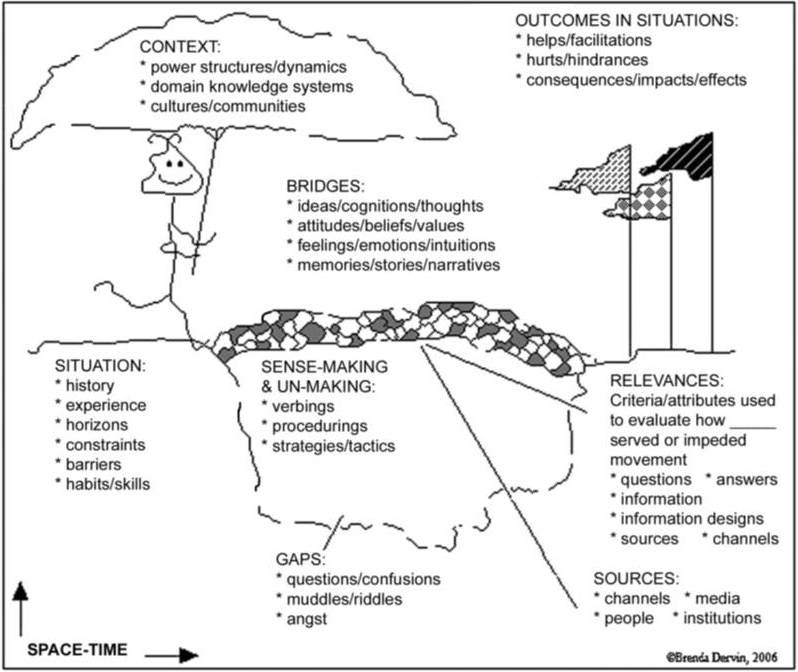
\includegraphics[width=.7\columnwidth]{dervin}
	\caption[The gap-bridging metaphor of sensemaking]{The gap-bridging metaphor of sensemaking. People encounter gaps while moving through time-space, then seek for information, evaluate and use it to bridge the gaps. \is{Dervin2012}}
	\label{fig:lr-dervin}
\end{figure}

\subsection{Sensemaking in Organizations}
Different from Dervin who studies sensemaking for individuals, Weick focuses on sensemaking at an organization level~\cite{Weick1995}. He proposes that sensemaking consists of these seven following properties.

\begin{enumerate}
	\item \emph{Grounded in identity construction}. Who people think they are, both individually and collectively, affect what they interpret and act.
	\item \emph{Retrospective}. People look back and make sense from what they have said and what they have done before.
	\item \emph{Enactive of sensible environments}. People make sense and contribute to the environments during their sensemaking processes.
	\item \emph{Social}. This is an inherent property of sensemaking in an organization where people interact and socialize with others, and are also influenced by others.
	\item \emph{Ongoing}. Sensemaking is continuous because the world and our understanding about it are constantly changing.
	\item \emph{Focused on and by extracted cues}. Cues are things that people have attention to and may use them to guide further exploration and assessment of the sensemaking problem.
	\item \emph{Driven by plausibility rather than accuracy}. Sensemaking focuses on plausibility and sufficiency rather than accuracy and completeness. People tend to stop searching when they find an acceptable solution.
\end{enumerate}

\subsection{Learning Loop Complex}
Russell~et~al.~\cite{Russell1993} define sensemaking as the process of searching for a representation and encoding data into that representation to answer task-specific questions. That cyclic process is called the \emph{learning loop complex} as illustrated in \autoref{fig:lr-russell}. First, the sensemaker (the person who is making sense of a problem) searches for a representation to capture salient features of the data (\emph{Generation Loop}). During sensemaking, new information is sought and encoded into this representation (\emph{Data Coverage Loop}). The data unfit to the representation (\emph{residue}) requires the sensemaker to adjust and to produce a more suitable one. This entire learning loop complex is guided by the task with an aim to reduce its cost.

\begin{figure}
	\centering
	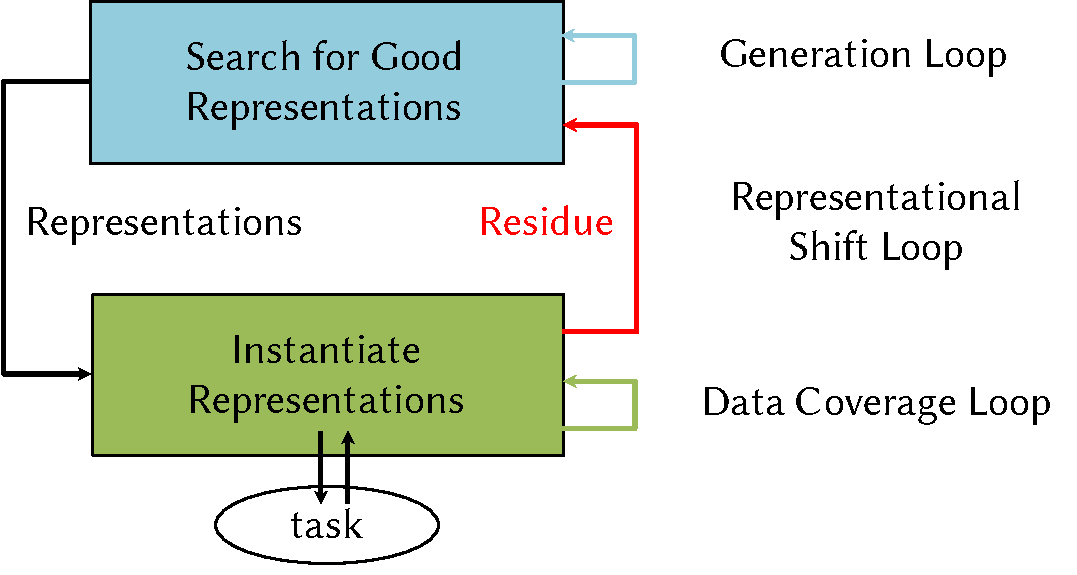
\includegraphics[width=.5\columnwidth]{russell}
	\caption[The learning loop complex theory of sensemaking]{The learning loop complex theory of sensemaking. It consists of three iterative loops: searching for a good representation, encoding data into the representation, and adjusting that representation for a better data coverage. These loops are guided by the task and the instantiated representations are then used to implement the task. \is{Russell1993}}
	\label{fig:lr-russell}
\end{figure}

\subsection{A Process Model}
\label{sub:lr-pcm}
Pirolli and Card~\cite{Pirolli2005} describe sensemaking as an iterative process that gradually transforms raw data into reasoning knowledge. The process includes two sets of activities: one that cycles around finding relevant information, and another that cycles around making sense of that information, with plenty of interaction between them. They map to the \emph{foraging loop} and the \emph{sensemaking loop} respectively, as shown in \autoref{fig:lr-pirolli-card-model}. The sensemaking process can progress upward (from data to knowledge) or downward (from knowledge to data). The steps in the \emph{bottom-up} process are summarized as follows.

\begin{figure}
	\centering
	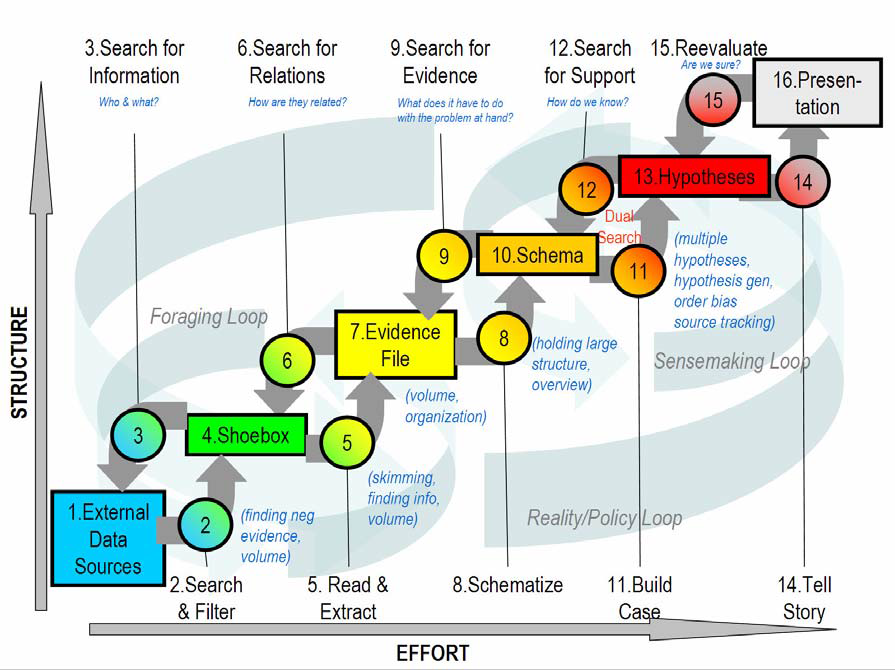
\includegraphics[width=.7\columnwidth]{pirolli-card-model}
	\caption[The Pirolli and Card's model of sensemaking]{A notional process model of sensemaking. The sub-processes (numbered circles) and their data input/output (numbered rectangles) are arranged in a two-dimensional space, in which the horizontal axis represents the degree of effort from users, and the vertical axis represents the degree of structure in information representation. \is{Pirolli2005}}
	\label{fig:lr-pirolli-card-model}
\end{figure}

\begin{itemize}
	\item \emph{Search and filter}. External data sources, such as classified databases or the web, are searched and filtered to retrieve relevant documents to the task.
	\item \emph{Read and extract}. These documents are examined to extract pieces of important information that may be used as evidence later.
	\item \emph{Schematize}.  The collected information is organized in a way that aids the analysis. This organization may be executed implicitly in one's mind, using paper and pen, or with support of a complex computer-based system.
	\item \emph{Build case}. Multiple hypotheses are generated, and evidence are marshaled to support or disconfirm them.
	\item \emph{Tell story}. Discovered cases are presented to some audience of interest.
\end{itemize}

In this model, \emph{schematization} plays an important role in converting raw evidence to reasoning explanations, bridging the foraging and sensemaking loops. A study by Kang, Görg and John Stasko~\cite{Kang2011} also agrees with this suggestion. In their study, all the participants who performed sensemaking tasks well spent considerable time and effort in organizing their collected information. Their organizational schemas were flexible: a \emph{timeline} of related events, a \emph{map} connecting locations that a person has been to, and a \emph{diagram} showing relationships among suspicious targets.

\subsection{Data--Frame Model}
\label{sub:lr-dfm}
Klein et al.~\cite{Klein2003} propose a sensemaking model that centers around data and frame. \emph{Data} is the information that a person receives or searches for, and \emph{frame} is the mental structure that organizes and explains the relationship of such data. For instance, a frame can be a \emph{story}, explaining the chronology of events and the causal relationships between them; or a \emph{map}, showing where the events take place and the routes between them. Sensemaking is considered as a deliberate effort to understand an event, starting when a person realizes a gap of their current understanding of that event. Klein and his associates describe seven activities involved in sensemaking and are summarized in \autoref{fig:lr-data-frame-model}.

\begin{figure}
	\centering
	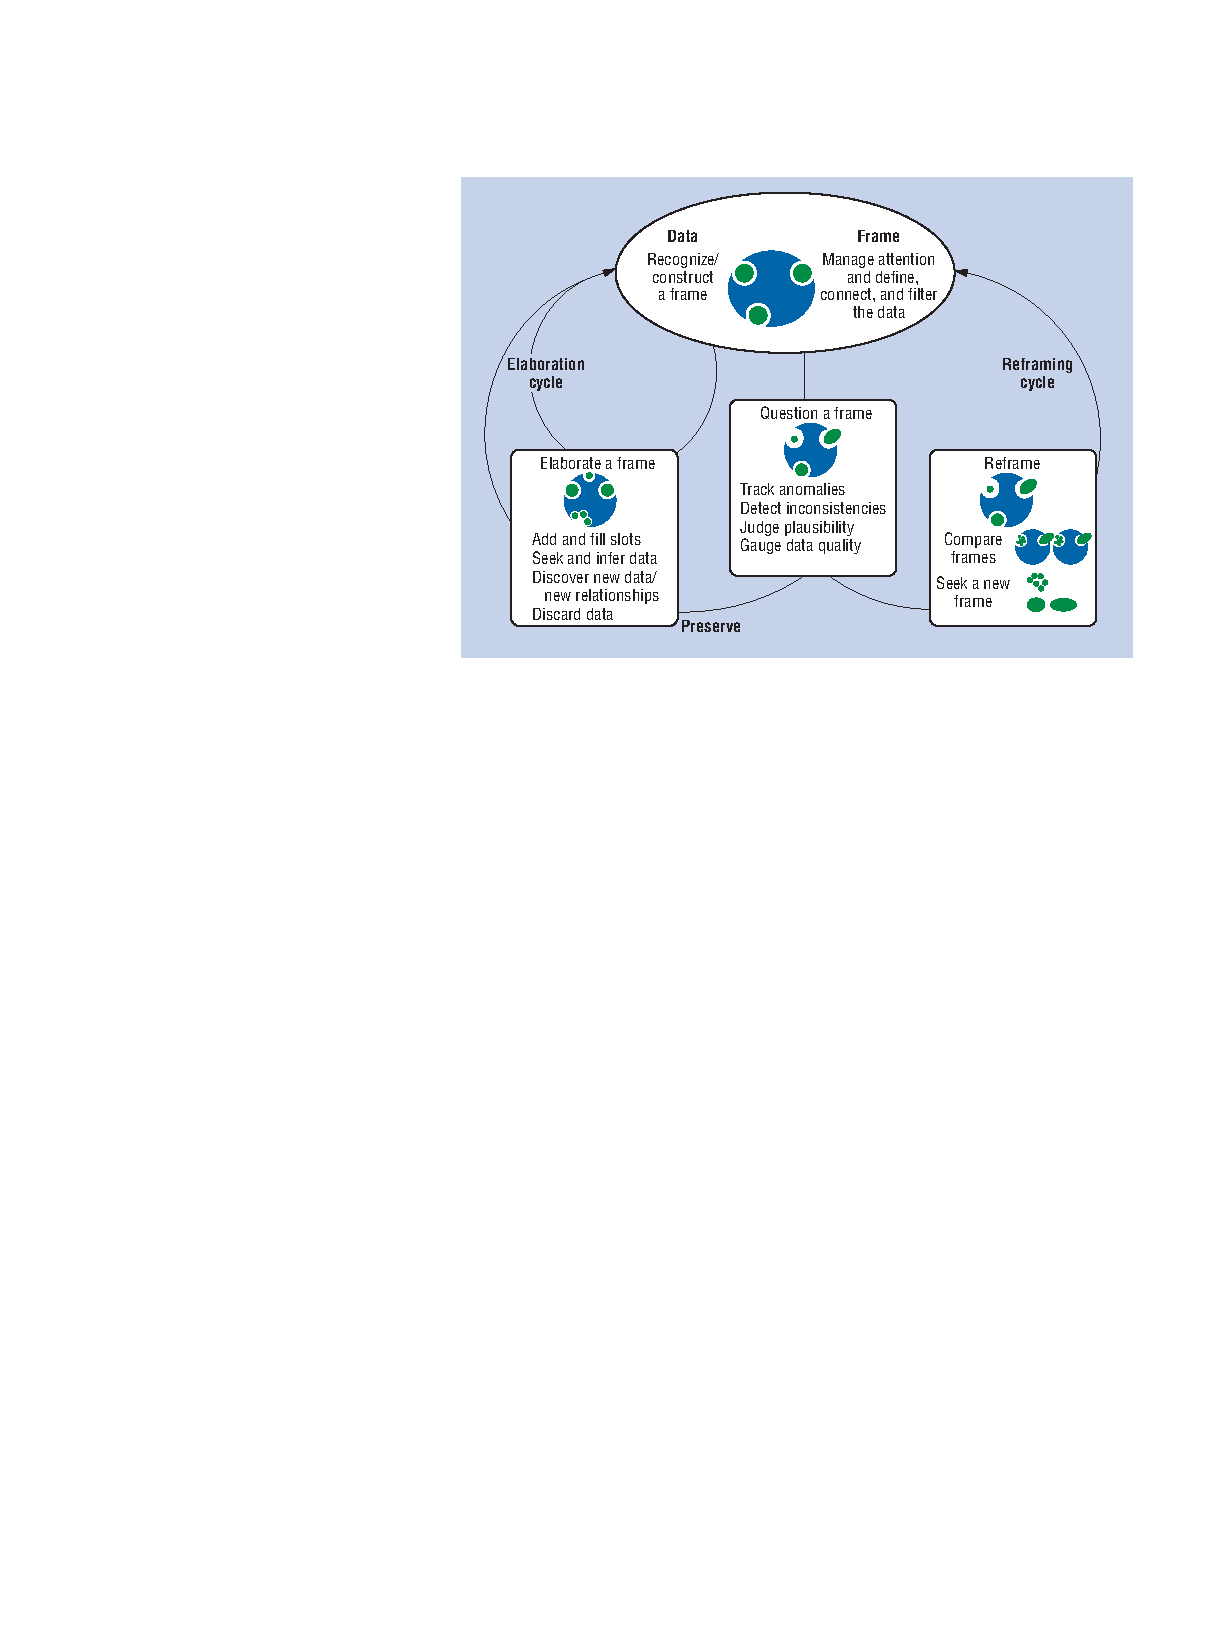
\includegraphics[width=.7\columnwidth]{data-frame-model}
	\caption[The data--frame model of sensemaking]{The data--frame model of sensemaking. It describes a set of interconnected sensemaking activities centering around data and frame -- the explanatory structure of data. \is{Klein2003}}
	\label{fig:lr-data-frame-model}
\end{figure}

\begin{itemize}
	\item \emph{Connect data and a frame}. A person recognizes relevant pieces of data and constructs an initial frame to explain them. The frame then helps the person filter and search for new data.
	\item \emph{Elaborate the frame}. As more is learned about the situation, the frame becomes more elaborate with new data and new relationships.
	\item \emph{Question the frame}. The question happens when a person encounters data that is inconsistent with the existing frame. At this point, the person may be unsure that the frame is incorrect, or the data is inaccurate.
	\item \emph{Preserve the frame}. A person may consider the severity of the inconsistent data, justify why it mismatches the frame, and ignore it.
	\item \emph{Compare multiple frames}. Depending on experience, a person may think of alternative frames explaining the same set of data. These frames need to be compared to select the most likely one.
	\item \emph{Reframe}. When encountering inconsistent and contrary data, a person may need to find a replacement to explain all data. Considering discarded data and/or reinterpreting data could facilitate this activity.
	\item \emph{Seek a new frame}. A person may deliberately search for a new frame when encountering plenty of conflicted data. One or two key data elements may serve as \emph{anchors} to help the person to elicit another frame.
\end{itemize}

The Pirolli and Card's model describes a step-by-step process of sensemaking, in which the analyst collects relevant data and eventually transposes it into reasoning answers. However, the various sensemaking activities in the Data--Frame model may explain the strategies used by the analyst more comprehensively.

\subsection{Summary}
Even though being conducted in different contexts, sensemaking research agrees on many common points. Dervin~\cite{Dervin1983} describes sensemaking as a deliberate effort to bridge the gap of knowledge that a person encounters while solving a problem. More specifically, Russell~et~al.~\cite{Russell1993} propose an iterative process of searching for an appropriate representation of data to bridge such a gap, or to reduce the cost of sensemaking operations. Klein et al.~\cite{Klein2003} make the representation shift more explicitly by describing seven different sensemaking activities between data and the representation, or frame. More completely, Pirolli and Card~\cite{Pirolli2005} suggest a process model of sensemaking that covers searching and filtering relevant information, organizing them, generating hypotheses and presenting the final outcome.

Supporting sensemaking is challenging because it usually happens implicitly inside a person's head. The aforementioned sensemaking models help unfold this tacit process and provide guidance for improvement. This thesis chooses the Pirolli and Card's model and the Data--Frame model as the theoretical foundation for sensemaking because of their comprehensive structure. \autoref{chap:schemaline} and \autoref{chap:timesets} focus on the schematization process and support all sensemaking activities in the Data--Frame model. \autoref{chap:sensemap} provides sensemaking support based on a simplified version of the Pirolli and Card's model. The support is achieved through the externalization and visualization of the implicit sensemaking process. To provide an overall understanding of the power of visualization, the next section will discuss its core concepts and research.